% !TEX encoding = UTF-8
% !TEX TS-program = pdflatex
% !TEX root = ../Lahmer_Abdelilah_tesi.tex
% !TEX spellcheck = it-IT

%**************************************************************
\chapter{L'azienda}
\label{cap:azienda}
%**************************************************************
\section{Profilo aziendale}
L'azienda presso la quale ho svolto il mio stage è Sopra Steria Group S.p.A, una delle imprese che propone una delle offerte più complete di servizi end to end presenti oggi sul mercato.\\

\begin{figure}[H]
	\centering
   	
\includegraphics[width=0.6\textwidth]{immagini/logo_azienda}
   	\caption{Logo di Sopra Steria Group S.p.A. - Fonte: sito internet dell'azienda}
\end{figure}

Sopra Steria è infatti tra i leader europei in ambito di trasformazione digitale, propone una delle più complete offerte di servizi di \textit{Consulting}, \textit{Systems Integration}, \textit{Software Development} e \textit{Business Process Services} presenti oggi sul mercato.
Essa spazia su diversi mercati come Fashion, Insurance, Banking, Retail, Energy, Aeronautica, Industria e Servizi, Sanità, Settore pubblico, Difesa e Trasporti.\\

Sopra Steria Group è partner di riferimento delle principali aziende ed organizzazioni pubbliche e private proponendo progetti di trasformazione di successo per affrontare al meglio le sfide di business più critiche e complesse, combinando un'alta qualità dei servizi erogati, valore aggiunto e innovazione.\\

L'azienda conta più di 40.000 collaboratori in più di 20 paesi, vanta inoltre un fatturato di 3,7 miliardi di euro nel 2016. Nello specifico opera sul territorio italiano con più di 800 risorse distribuite nelle sue sedi di Ariano Irpino (AV), Assago (MI), Asti, Collecchio (PR), Padova e Roma, fatturando circa 56,9 milioni nel 2016 .\\

%\begin{figure}[H]
%	\centering
%   	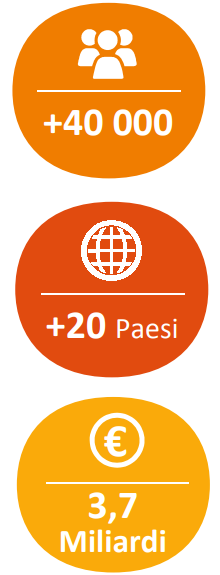
\includegraphics[width=0.2\textwidth]{immagini/dipendenti_paesi_fatturato_mondo}
%   	\caption{Informazioni generali - Fonte: documento interno aziendale}
%\end{figure}

%\begin{figure}[H]
%	\centering
%   	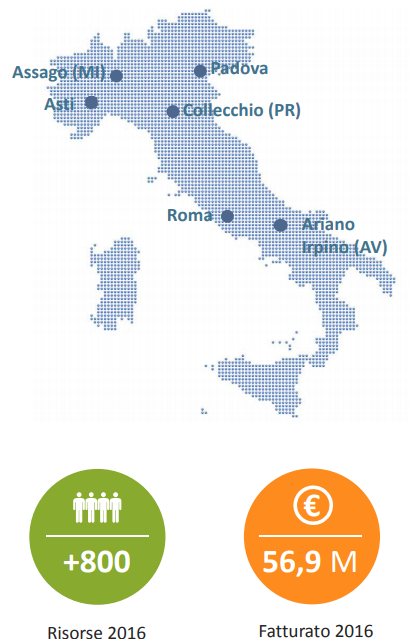
\includegraphics[width=0.4\textwidth]{immagini/mappa_italia_fatturato}
%   	\caption{Mappa italiana - Fonte: documento interno aziendale}
%\end{figure}

\begin{figure}[htbp]
\centering
\begin{minipage}[c]{.40\textwidth}
\centering\setlength{\captionmargin}{0pt}%
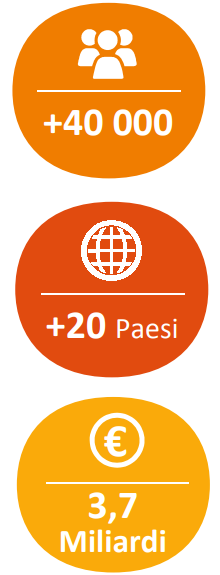
\includegraphics[width=0.6\textwidth]{immagini/dipendenti_paesi_fatturato_mondo}
\caption{Dati generali Sopra Steria nel Mondo}
\end{minipage}%
\hspace{10mm}%
\begin{minipage}[c]{.40\textwidth}
\centering\setlength{\captionmargin}{0pt}%
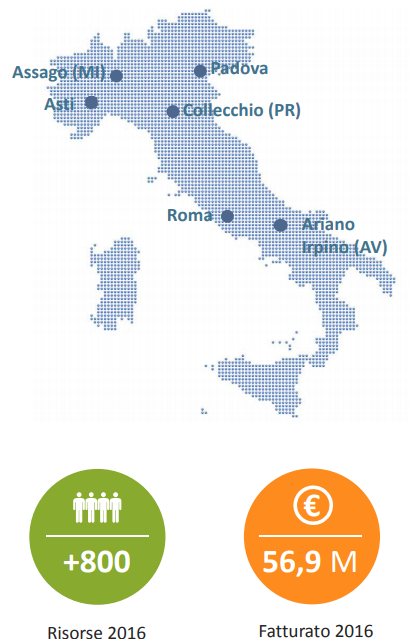
\includegraphics[width=1.2\textwidth]{immagini/mappa_italia_fatturato}
\caption{Dati generali Sopra Steria in Italia}
\end{minipage}
\caption{Informazioni generali Sopra Steria Group S.p.A. - Fonte: documento interno aziendale}
\end{figure}


Il gruppo è il risultato di una fusione, avvenuta nel 2014, ad opera di due aziende francesi Sopra Group SA e Groupe Steria SCA, comunemente chiamate Sopra e Steria, fondate rispettivamente nel 1968 e 1969. Ad oggi l'azienda si presenta internamente ben strutturata in \textit{Business Unit} relative agli ambiti di sviluppo e adotta una politica di recruiting che mira alla competenza dei dipendenti da cui deriva la qualità dei prodotti, punto di forza dell'azienda.\\

Io sono stato inserito nella divisione "793 - Servizi Finanziari e Assicurazioni" della sede di Padova, nata negli ultimi anni a partire da pochi dipendenti e che ora conta circa 20 dipendenti solo per la sede in cui ho avuto il piacere di collaborare, senza contare i colleghi situati nelle sedi di Collecchio e Roma che collaborano anch'essi agli stessi progetti per la stessa divisione.\\
In particolare il mio ruolo è stato quello del programmatore back-end e analista funzionale, sono stato affiancato quindi da vari colleghi a seconda della tecnologia o conoscenza che dovevo apprendere. \\
Più nello specifico sono stato affiancato dal mio collega Stefano Gori e dal mio tutor aziendale Marco Valentino, uno dei principali sviluppatori back-end e manager di prossimità di questa sede, per l'apprendimento dei linguaggi COBOL e JCL. Sono stato invece affiancato dalle mie colleghe Chiara Maccotta e Francesca Constantini per l'apprendimento dei concetti teorici in ambito economico.% essenziali per poter aver un quadro generale di quale sia lo scopo pratico del prodotto su cui si lavora e di una base teorica che permetta di raggionare sui risultati ottenuti dopo implementazioni e rispettivi risultati ottenuti.

%Da questo punto le descrizioni delle caratteristiche aziendali faranno riferimento alla divisione sopra citata dal momento che ognuna di esse opera secondo logiche, ambiti e tecnologie differenti.

%**************************************************************
\section{Prodotti e servizi offerti}
	
	\subsection{Prodotti}
	
	Nei mercati francesi, dove l'azienda è radicata, è attiva la vendita di prodotti bancari, ovvero software già pronto e configurabile in poco tempo presso il cliente. In Italia la situazione è differente e per i principali clienti, nell'ambito finanziario, raramente si vendono pacchetti di prodotti finiti ma si adotta una politica di personalizzazione secondo le esigenze del cliente. I prodotti principali offerti dalla business unit in cui sono stato formato sono quindi riassumibili in:
		
	\begin{itemize}
		\item Applicazioni web per la gestione di finanziamenti bancari e la relativa evoluzione e manutenzione;
		\item Programmi \textit{host} di gestione dati e della loro consistenza e persistenza.
	\end{itemize}
	
	\subsection{Servizi}
	
	Il sistema di gestione per la qualità dei servizi offerti ai clienti di Sopra Steria Group è certificato ISO 9001:2008 ed è annualmente sottoposto a verifiche da parte di un ente accreditato di terza parte. I principali servizi erogati dalla divisione per l'ambito bancario sono:
	
	\begin{itemize}
		\item Consulenza in ambito informatico per l'ampliamento ed il soddisfacimento della clientela da parte dei commerciali;
		\item Analisi delle necessità del cliente e dei conseguenti requisiti software;
		\item Progettazione e realizzazione di nuove applicazioni o nuove funzionalità di applicativi già in uso;
		\item Verifica e collaudo del software prodotto con finale rilascio nei sistemi del cliente;
		\item Manutenzione dei contenuti proposti al cliente in un'ottica a lungo termine.
	\end{itemize}

%**************************************************************
\section{Processi aziendali}

	\subsection{Organizzazione interna}
	
	Le grandi dimensioni dell'azienda implicano una forte strutturazione interna e un'attenta gestione delle attività di coordinamento. Durante il mio stage ho avuto modo di osservare alcuni aspetti di questo complesso sistema.\\
	
	Una delle prime cose che si imparano di quest'azienda è la sua propensione alla cura dei rapporti con il cliente, poiché vengono offerte numerose sessioni	di consulenza. La filosofia è quella di collaborare per aiutarli a trasformare i loro sistemi informativi e, grazie all'esperienza del settore, offrire valore aggiunto mediante le soluzioni. Per raggiungere tale scopo il gruppo ha stretto delle partnership strategiche con Microsoft, IBM, Oracle e HP. La missione principale del gruppo è di industrializzare e ottimizzare le proprie operazioni per migliorare la competitività e le performance in un'ottica a lungo termine.\\
	
	Un altro aspetto a cui l'azienda tiene in particolar modo è la gestione delle risorse umane. Anticipare e sostenere lo sviluppo dell'evoluzione di queste ultime è considerata	una priorità per il successo aziendale e per mantenere un alto livello di soddisfazione e di motivazione dei dipendenti. Per questo Sopra Steria si impegna a conoscere i profili e le competenze di ciascun collaboratore, al fine di poter offrire agli stessi prospettive di crescita e percorsi di carriera in grado di soddisfare sia le loro aspettative che il mercato.\\
	
	%La crescente complessità dei progetti, la molteplicità degli interlocutori e le esigenze di alto livello dei clienti sono tali da comportare rischi considerevoli per l'azienda. L'intervento della direzione legale si rende pertanto necessario per difendere al meglio gli interessi del gruppo, tutelando i rapporti contrattuali con i clienti e le fasi di contenzioso, i rapporti con le software house, le parti terze, i partner e i fornitori e le acquisizioni o cessioni di attività.
	
	Per quanto riguarda il governo e la gestione del gruppo, i diversi livelli di poteri decisionali, sia a livello funzionale che produttivo, sono distribuiti nella gerarchia operativa oltre che nella direzione. Alla base di ciò, un'organizzazione complessa si ramifica nelle varie nazioni in cui l'azienda si estende, delegando l'amministrazione di questi filoni e di altri reparti di supporto a manager selezionati. A livello più basso si collocano le Business Unit, ovvero le varie divisioni aziendali adibite all'erogazione di determinate tipologie di prodotti e servizi identificate anche in base al mercato di riferimento. Anche queste ultime risultano distribuite nel territorio, in ogni filiale infatti possono coesistere più reparti.\\
	
	\begin{figure}[H]
	\centering
	   	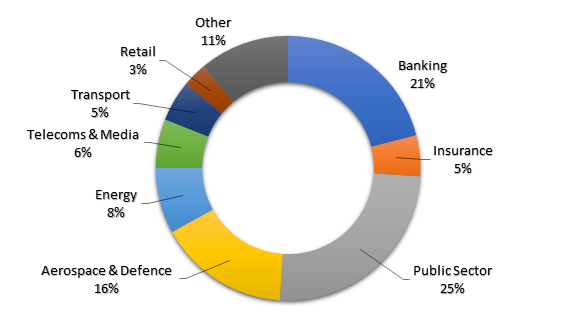
\includegraphics[width=0.8\textwidth]{immagini/mercati_principali}
	   	\caption{Suddivisione dell'azienda nei vari mercati}
	\end{figure}
	
	Nella divisione in cui sono stato collocato vi sono diverse figure che si occupano dei vari processi di produzione. In ordine gerarchico è presente un direttore di Business Unit per l'amministrazione delle risorse della divisione, i project manager per la gestione dei progetti e dei loro costi, i commerciali che si occupano delle relazioni con i clienti in ambito di redazione dei contratti, i team di analisti e consulenti che si occupano dei requisiti del cliente e i team di sviluppo software, suddivisi in programmatori web e sviluppatori \textit{host}.\\
	
	L'azienda adotta un sistema di qualità anche per i suoi funzionamenti interni, in particolare è applicato per:
	
	\begin{itemize}
		\item Gestire i processi di prevendita e sviluppo di progetti e servizi;
		\item Gestire le risorse umane nel campo di reclutamento, carriera, gestione delle competenze, formazione interna e comunicazioni interne;
		\item Gestire e monitorare i processi aziendali, garantendo una manutenzione interna.
	\end{itemize}
	
	Sopra Steria si fa carico inoltre delle responsabilità d'impresa negli ambiti di uno sviluppo sostenibile, cura dell'ambiente, diritti umani e del lavoro e nel favorire le uguali opportunità. La pubblicazione del rapporto di tali attività fa parte di un processo di trasparenza, correttezza e dialogo con gli \textit{stakeholder}: collaboratori, clienti, azionisti, fornitori, partner e attori della società civile.
	\newpage
	\subsection{Modello Incrementale}
	
	Il ciclo di sviluppo software adottato da Sopra Steria nella divisione dei Servizi Finanziari è un'implementazione del modello incrementale, questa scelta è dovuta al fatto che l'azienda tratta per la maggior parte progetti già avviati, che richiedono aggiunte sulla base delle funzionalità essenziali già sviluppate. \\
	
	I punti di forza del procedimento incrementale sono i seguenti:
	\begin{itemize}
		\item L'integrazione delle parti del sistema è distribuita nel tempo e non collassata nelle fasi finali;
		\item Ogni incremento porta valore aggiunto, con lo sviluppo di nuove funzionalità e il soddisfacimento di alcuni requisiti;
		\item Ad ogni incremento si guadagnano esperienza e affidabilità, riducendo i rischi di fallimento;
		\item Le funzionalità essenziali sono sviluppate nei primi incrementi e attraversano più fasi di verifica, diventano quindi più stabili con ciascuna iterazione;
	\end{itemize}
	
	Questo modello si presta bene alle necessità dell'azienda perché i clienti richiedono che vengano effettuati lavori di manutenzione e amplificazione definibili in attività distinte, assimilabili facilmente tramite un ciclo di sviluppo ad incrementi. In figura vengono rappresentate le fasi del modello.\\
	
	\begin{figure}[H]
		\centering
	   	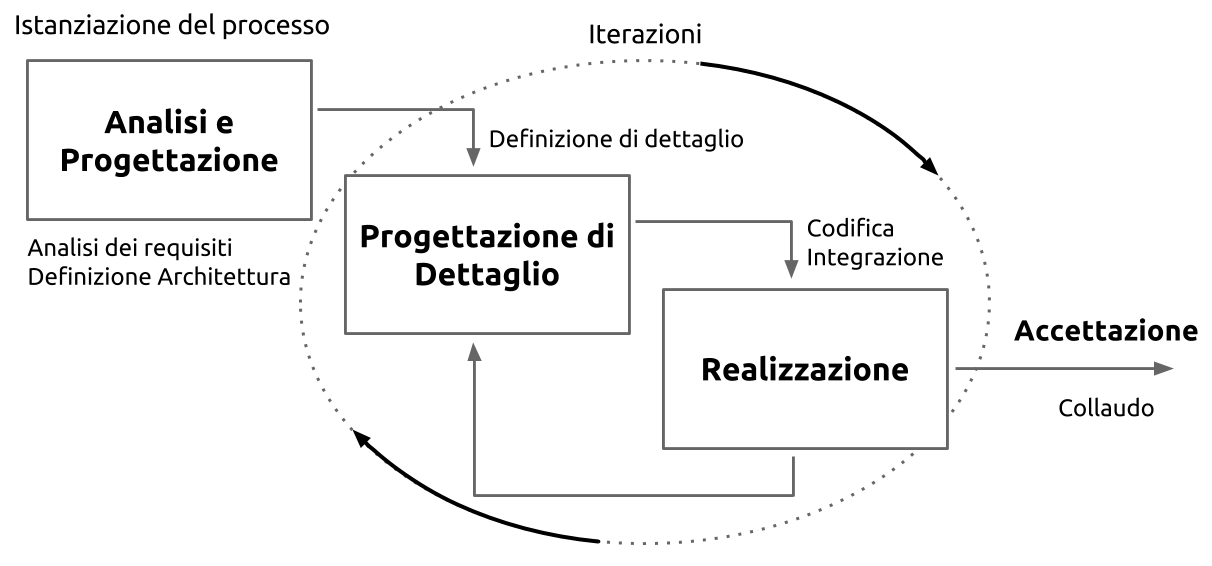
\includegraphics[width=1\textwidth]{immagini/modello_incrementale}
	   	\caption{Diagramma del modello di sviluppo incrementale}
	\end{figure}
	\newpage
	
	Il modello incrementale è un ciclo di sviluppo definito dallo standard ISO 12207 che combina la logica del modello a cascata, dove ogni fase è rigidamente sequenziale, e la filosofia iterativa della prototipazione.\\
	
	È prevista una prima fase di analisi dei requisiti fondamentali e di progettazione architetturale intesa a stabilire le fondamenta del software. Tale fase è essenziale per definire i successivi incrementi e non si ripete.\\
	
	Le fasi successive di realizzazione incrementale vera e propria, possono ripetersi più volte e mirano ad attività di progettazione di dettaglio,
	codifica e prove, in cui vengono trattati prima i requisiti essenziali e poi quelli desiderabili. Le implementazioni subiscono i trattamenti di 
	integrazione e collaudo, successivamente avviene un eventuale rilascio.\\

	È prevista la prototipazione delle nuove funzionalità che si vanno ad implementare per la validazione complessiva del sistema, reiterando 
	alle fasi di progettazione e realizzazione in caso di errori o problematiche. In questo modo è possibile di volta in volta acquisire maggiore competenza riguardo al problema, riducendo i rischi successivi e le tempistiche globali di produzione software.
	
	\subsection{Il modello incrementale in Sopra Steria}
	
	Ogni ciclo di incremento inizia con la raccolta e l'analisi dei requisiti presso il cliente, che espone le sue necessità tramite riunioni oppure mediante opportuna documentazione.\\
	
	Gli analisti a questo punto si occupano di raggruppare i requisiti in macro attività, calcolare le tempistiche necessarie per il loro completamento e stilare i documenti di analisi funzionale e specifica tecnica per ognuna di esse, dov'è compresa la progettazione di dettaglio. Tale documentazione risulta necessaria ai vari team di sviluppo per la comprensione e l'applicazione delle implementazioni richieste.\\
	
	Gli analisti rimangono a disposizione degli sviluppatori anche nelle fasi successive per eventuali chiarimenti e specificazioni, in modo da non rallentare o interrompere le fasi successive. I documenti vengono inviati ai team competenti a cui sono state attribuite le macro attività e da quel momento inizia la realizzazione. Tali gruppi di lavoro possono risultare distribuiti nelle varie sedi del territorio italiano, perciò sono previste molte comunicazioni telefoniche o tramite posta elettronica e occasionali trasferte; al fine di allineare le procedure di sviluppo o rendere noto quando è possibile procedere con determinate modifiche. \\
	
	L'evoluzione degli incrementi software attraversa ambienti distinti in base alle mansioni svolte su di essi. Esistono in particolare i seguenti ambienti:
	\begin{itemize}
		\item \textbf{Sviluppo}: ambiente di programmazione locale, qui avviene l'implementazione delle modifiche software;
		\item \textbf{Integrazione}: in questo ambiente vengono raccolte le implementazioni delle attività e si verifica che non generino conflitti, garantendo la stabilità del sistema;
		\item \textbf{Collaudo}: ambiente di validazione delle funzionalità complessive del software, utilizzato anche per dimostrare al cliente la loro consistenza;
		\item \textbf{Produzione}: questo ambiente varia per ogni cliente o applicazione sviluppata e rappresenta lo stato finale del prodotto in cui viene effettivamente utilizzato dal cliente.
	\end{itemize}	
	
	È responsabilità del programmatore che prende in carico lo sviluppo delle funzionalità dichiarare il loro completamento, almeno a livello di prototipo, per rilasciarlo in integrazione. Determinati team si occupano poi di testare l'applicazione nelle sue nuove funzioni, accertando il soddisfacimento dei requisiti ed eventualmente contattando gli analisti per eventuali modifiche progettuali. In caso di problematiche le modifiche vengono respinte in ambito di sviluppo altrimenti vengono approvate per il collaudo. In collaudo è possibile utilizzare le funzioni sviluppate da altri team e validare il lavoro svolto per presentarlo poi al cliente, rilasciando in produzione la nuova versione del software.
	
	\subsection{Strumenti a supporto di processi e servizi}
	
	\subsubsection{Linguaggi}
	Sviluppando principalmente applicativi web, nella Business Unit in cui ho svolto il tirocinio è stata adottata la piattaforma Java per il web (Java EE) e ovviamente le tecnologie standard relative alla presentazione e al comportamento delle pagine.\\
	
	Ho utilizzato quindi anche HTML, CSS e JavaScript che nella quasi totalità dei casi sono generati dinamicamente lato server tramite pagine JSP.\\
		
	Java Platform Enterprise Edition, o Java EE, è un'estensione di Java SE (Standard Edition) e rappresenta una piattaforma di sviluppo software molto usata per applicazioni d'impresa. Java EE è mantenuto mediante il Java Community Process ovvero un processo che permette ad una comunità di esperti industriali,	organizzazioni (commerciali e \textit{open source}) e ad un incredibile numero di individui di dare il loro contributo seguendo determinati standard. Esso fornisce gli strumenti utili per la programmazione Web, tra cui un ambiente \textit{runtime} e librerie utili allo sviluppo di applicazioni distribuite, scalabili, affidabili e sicure che prevedono Java come linguaggio di programmazione primario.
	
	\begin{figure}[H]
		\centering
	   	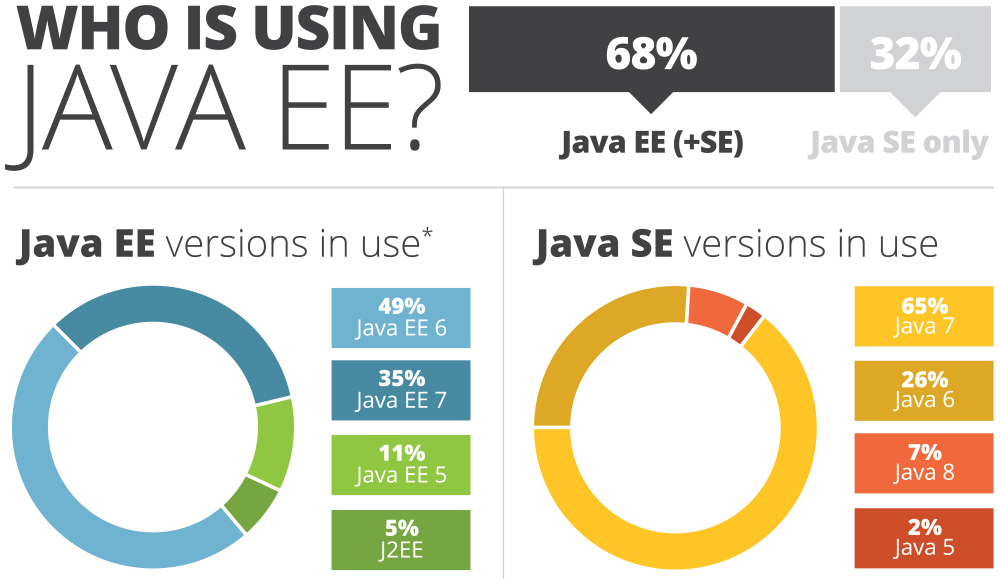
\includegraphics[width=0.8\textwidth]{immagini/utilizzi_java}
	   	\caption{Utilizzi della piattaforma Java nelle sue versioni - Fonte: RebelLabs}
	\end{figure}	
	
	\subsubsection{Framework}
	Per definire la spina dorsale delle applicazioni web, invece, l'azienda utilizza diversi framework tra cui Struts, Maven e Hibernate. Apache Struts è un framework \textit{open source}, usato nel progetto di stage, per lo sviluppo di applicazioni web su piattaforma Java EE, gestisce le richieste client e smista il flusso applicativo in base alla logica configurata mediante file XML, dove vengono definite le associazioni tra i vari elementi che compongono il sistema, sotto forma di \textit{action}.\\
	
	\begin{figure}[H]
		\centering
	   	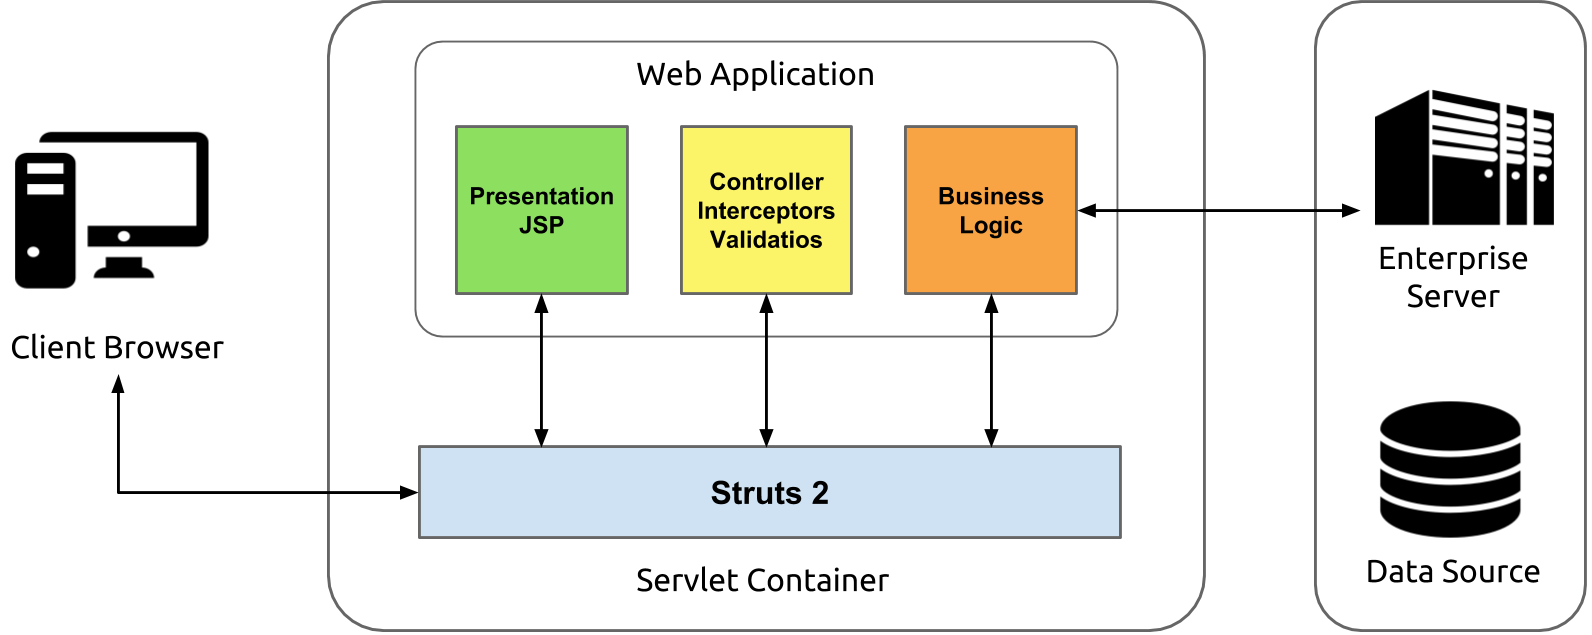
\includegraphics[width=1\textwidth]{immagini/architettura_struts}
	   	\caption{Architettura di un'applicazione web che adotta il framework Struts}
	\end{figure}	
	
	L'utilizzo di Struts permette lo sviluppo di applicazioni web di notevoli dimensioni, inoltre agevola la suddivisione dello sviluppo del progetto fra i vari dipendenti. I programmatori web e i vari gruppi di sviluppatori possono quindi gestire in parallelo e autonomamente la loro parte del progetto.
	
	\subsubsection{Database e applicazioni host}
	Il salvataggio dei dati per le applicazioni in ambito bancario e assicurativo avviene solitamente tramite DBMS\glossario\ relazionali come DB2 dell'IBM, Microsoft SQL Server e MySQL di Oracle. DB2 è nato nel 1983 ma tutt'oggi è uno tra i DBMS più usati, specie in questo settore. In origine era nato come DBMS per i mainframe CICS\glossario\, poi si è diffuso su qualsiasi tipo di server. Per questo banche e assicurazioni, enti che esistono da molto prima, inizialmente hanno adottato questa tecnologia mediante sistemi EIS\glossario\ implementati in linguaggio COBOL\glossario\ che tutt'oggi gli forniscono le funzionalità necessarie senza il bisogno di adottare tecnologie più recenti e sviluppate secondo le esigenze dei moderni paradigmi di programmazione.\\
	
	%Esso supporta il modello relazionale, ma negli ultimi anni è stato esteso il supporto a funzionalità ad oggetti e non relazionali come JSON e XML.\\
	
	Microsoft SQL Server e MySQL di Oracle sono utilizzati come soluzioni secondarie per la gestione di dati in sola lettura di natura statica.
	%MySQL è un DBMS open source nato nel 1995 che mette a disposizione delle interfacce grafiche.
		
	\subsubsection{Gestione di progetto}
	A supporto della gestione delle attività progettuali e dell'organizzazione delle comunità aziendali, Sopra Steria mette a disposizione dei suoi dipendenti un portale comune dove poter ottenere informazioni sulla vita aziendale e la gestione dei gruppi di lavoro. \\
	
	Il portale aziendale, Face2Face, gestisce molteplici attività e problematiche. Tramite esso i dipendenti sono tenuti a riportare settimanalmente le proprie attività di lavoro e gli ambiti di progetto al fine di inviare i dati alla direzione, permettendole di coordinare le risorse a disposizione. Il sito consente inoltre di consultare le news aziendali e gli eventi organizzati, come ad esempio i corsi di formazione interna a cui gli sviluppatori sono invitati a partecipare.

	\begin{figure}[H]
		\centering
	   	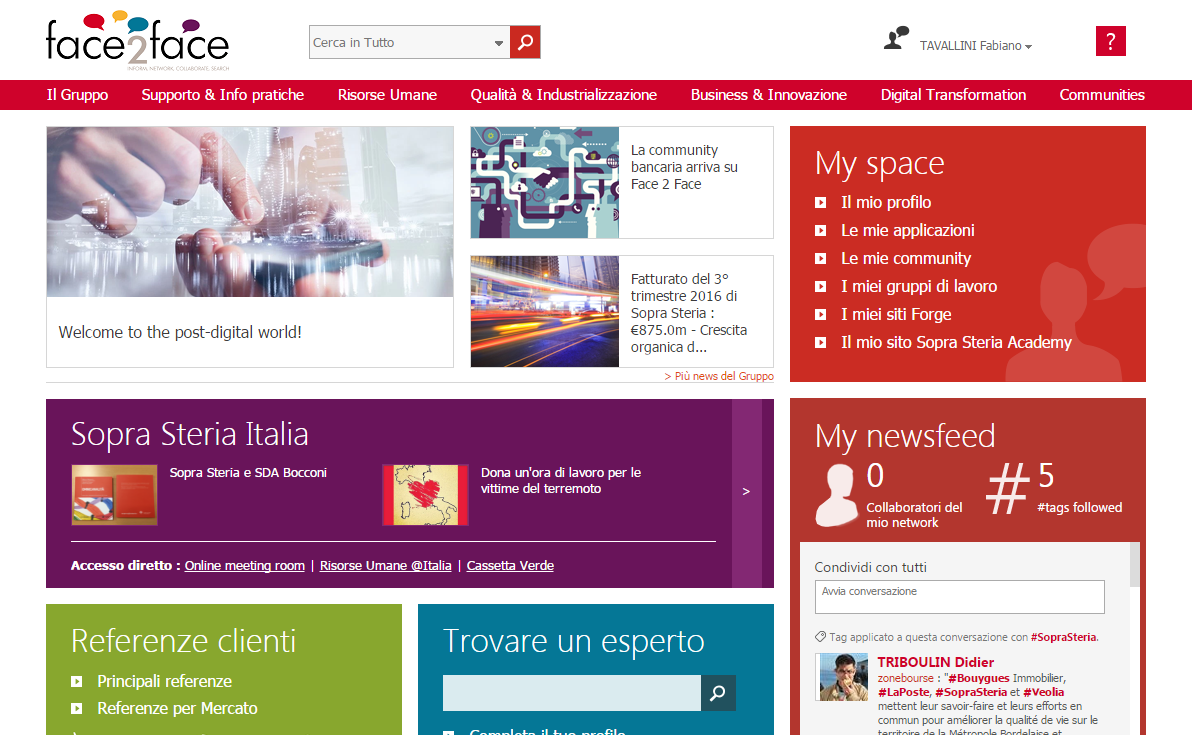
\includegraphics[width=0.9\textwidth]{immagini/face2face}
	   	\caption{La pagina iniziale di Face2Face - Fonte: portale interno dell'azienda}
	\end{figure}
		
	Face2Face è accedibile anche da rete remota come anche il sistema di posta elettronica, facilitando il lavoro in trasferta, e consente anche di inviare ai tecnici informatici segnalazioni riguardo i propri strumenti di lavoro per ricevere assistenza.\\
	
	Oltre a questo, i vari team di progetto comunicano molto spesso via email utilizzando Microsoft Outlook e telefonicamente per coordinarsi nei lavori. I capi progetto inoltre mantengono l'organizzazione delle attività, confrontandosi con gli analisti, utilizzando Microsoft Excel come strumento di supporto e stesura dei piani di lavoro.
	
	\subsubsection{Documentazione}
	Per ogni attività risultante dall'analisi dei requisiti vengono redatti due documenti: l'Analisi Funzionale e la Specifica Tecnica.
	Il primo affronta i requisiti ad alto livello, enunciando le principali funzionalità ed i cambiamenti rispetto alla versione attualmente in produzione dell'applicativo. \\
	
%	//Le sezioni principali di questo documento sono:
%	//- Matrice dei requisiti: enunciato discorsivo per introdurre il problema proposto;
%	//- Descrizione funzionale: per spiegare il comportamento dell'applicativo lato web, presentatando anche un'anteprima delle pagine che verranno aggiunte;
%	//- Casi oggetti di collaudo: qui vengono indicate le componenti che saranno analizzate in fase di testing per verificarne il corretto comportamento;
%	//- Dettaglio tecnico: qui vengono segnalate solo alcune particolarità e vengono enunciate le componenti software che saranno modificate o aggiunte.	
	
	Il secondo documento affronta nel dettaglio gli aspetti tecnici che vanno modificati o aggiunti trattando principalmente i programmi COBOL\glossario\ lato \textit{host}, dai quali poi anche i programmatori web possono individuare i parametri da utilizzare nelle richieste via rete per recuperare i dati e quindi allinearsi. Si può quindi dire che per la programmazione delle interfacce risulta di primaria importanza il primo documento. \\
	
	Al termine dello sviluppo dei requisiti, ad avvenuta validazione, viene inoltre redatto un documento di collaudo da consegnare al cliente per accertare i lavori eseguiti. \\
	
	Il software utilizzato per la produzione dei documenti è Microsoft Word, i cui formati sono standard sia per l'azienda che per i clienti.
	
	
	\subsubsection{Sistemi di versionamento}
	\label{sistemi-versionamento}
	Nei diversi prodotti software che la Business Unit ha sotto la propria responsabilità vengono utilizzati principalmente due sistemi di versionamento del software: 
	\begin{itemize}
		\item \textbf{SVN (Subversion, Apache)}: è un software di versionamento del codice distribuito gratuitamente sotto licenza Apache. E' ampiamente usato e sviluppato da una comuinità	globale di collaboratori. Offre alcune funzionalità chiave per chi lo sceglie come \textit{commit} visti come operazioni atomiche, operazioni di \textit{branch}, \textit{changelists} e design client-server;
		\item \textbf{RTC (Rational Team Concert, IBM)}: è costruito su IBM Jazz, una piattaforma estensibile che aiuta i team a integrare i task attraverso il ciclo di vita del software.	Ha un'architettura client-server e permette ai team di sviluppo di tenere traccia del loro lavoro tramite \textit{work items}, \textit{source control}, \textit{reporting} e \textit{build management} in un singolo ambiente.
	\end{itemize}
	
	\subsubsection{Ambienti di sviluppo}
	Il principale ambiente di sviluppo adottato per le applicazioni web è Eclipse. Esso racchiude la globalità delle caratteristiche necessarie ad uno sviluppatore in questo ambito.\\	
	
	Rappresenta un'ottima soluzione e agevolazione per il processo di sviluppo, in quanto offre funzionalità di collegamento ai sistemi di versionamento, \textit{debugging} del codice \textit{runtime} e avvio del software mediante gli \textit{application server} che si desidera installare, oltre alle molteplici caratteristiche offerte dai comuni editor di testo orientati allo sviluppo dei sorgenti software.
	
	\begin{figure}[H]
		\centering
	   	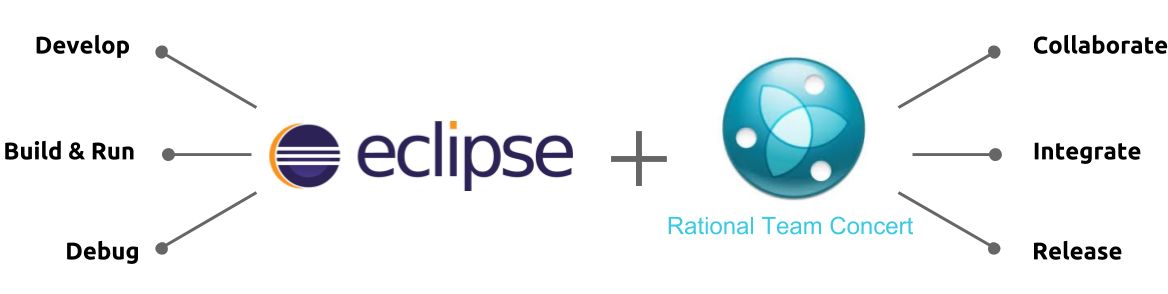
\includegraphics[width=1\textwidth]{immagini/ambienti_sviluppo}
	   	\caption{I vantaggi dell'uso di Eclipse in collaborazione con RTC}
	\end{figure}
	
	Altri programmi di supporto sono invece i diversi browser in cui bisogna testare il funzionamento delle pagine web tra cui Internet Explorer, Firefox e Chrome e gli editor di testo utili in situazioni dov'è richiesta più praticità come Notepad++.
	
	\subsubsection{Sistemi operativi}
	Per le postazioni di sviluppo è previsto un sistema centralizzato di utenze a cui è attribuito un proprio ambiente di lavoro ed uno spazio assegnato a cui accedere da qualsiasi computer aziendale.\\
	
	Nelle macchine aziendali è consueto l'utilizzo di Windows 7 come sistema operativo primario per ovviare a discrepanze nelle postazioni dei diversi dipendenti e per omogenizzare ulteriormente il processo di sviluppo. Questo comporta una buona soluzione per concentrarsi unicamente sul proprio lavoro e avere al contempo una garanzia nell'utilizzo quotidiano.
	
%**************************************************************
\section{Clientela e trasformazione digitale}

	\subsection{Target}
	
	I target di Sopra Steria, per quanto riguarda la divisione dei Servizi Finanziari e Assicurazioni, sono principalmente gruppi bancari e assicurativi. Essi necessitano una qualche forma di innovazione o evoluzione che le garantisca continuità di produzione ma anche i corretti adeguamenti previsti dai cambiamenti legislativi.\\
	
	 Per permettere questo, gli analisti si incaricano di entrare in contatto con i responsabili ICT\glossario\ della società cliente, dai quali poi si ricavano diverse richieste implementative; dalla variazione di	qualche caratteristica alla creazione di funzionalità completamente nuove interne o meno all'applicativo che essi adottano. 
	
	\subsection{Innovazione}
	
	L'innovazione in ambito bancario e assicurativo rappresenta uno scoglio non indifferente, in quanto questi enti sono da sempre legati a tecnologie primordiali come il linguaggio COBOL\glossario\ e la relativa implementazione in mainframe CICS\glossario : si è preferito infatti non migrare da essi o evolvere in altra tecnologia software.\\
	
	Per l'azienda, che fa della trasformazione digitale la sua bandiera, questo rappresenta una sfida e desidera mettersi in gioco offrendo le soluzioni adeguate, tenendo conto delle priorità del cliente e delle sue possibilità. Queste caratteristiche sono molto ricercate dalle aziende che vogliono rinnovarsi, trasformando i loro processi e servizi nel mondo digitale, adeguandosi ai moderni canoni di utilizzo e facendosi avanti nei mercati, con la possibilità di offrire prodotti di maggiore qualità e raggiungere molti più clienti.\\
	
	Fortunatamente per quanto riguarda il fornt-end\glossario\ degli applicativi, l'innovazione si fa strada mediante l'utilizzo di tecnologie adatte alla presentazione dei contenuti	nel web e di conseguenza maggiormente inclini a spinte evolutive dovute alla modernizzazione degli standard. Lo sviluppo di nuovi requisiti imposti dai clienti, inoltre, è sempre gestito in un'ottica che mira all'aggiornamento, anche per quanto riguarda le tecnologie e le loro versioni di utilizzo, per garantire, dove possibile, una futura compatibilità dove possibile.